%%%%%%%%%%%%%%%%%%%%%%%%%%%%%%%%%%%%%%%%%%%%
\subsubsection{MCS installation to the Telescope [Daytime]}\label{secflow:MCSinstall}

In this process, MCS is installed to the Cassegrain (Cs) Focus of the Subaru telescope.
MCS is attached to MCBox, which is installed to the flange of the Cs focus. 
This means that the MCS position is determined by how accurate MCBox is attached to the Cs focus.
The requirement {\tt REQ-MET-9} demands the accuracy of the MCS position with respect to the optical axis; decenter within 45mm (x/y each), and tilt within 0.14 degree.
Subaru demonstrated the repeatability of mounting MCBox in 2015 (report by Y. Minowa: {\tt NDTN-20150714}\footnote{MCBox\_repeatability\_report.pdf}), resulting in the following performance:
\begin{itemize}
\item Tilt: $<$ 10 arcsec
\item Shift(X,Y): $<$ 50um
\item Shift(Z): $<$ 0.5mm
\item Rot. : 0.0015 degree (shift by 0.24 um at the edge of MCS FoV)
\end{itemize}
This result implies the MCS will be installed well within the required accuracy, if it is installed in the normal way.
Note that we don't measure the repeatability indeed in the commissioning processes.
We will, however, have to check this process later, when a problem will happen; e.g. the center of PFI on MCS are quite different in individual runs.

%\bluetext{
%In this step, it should be also confirmed that flange, I/F of MCBox and M1, and CMOS sensor is parallel (Fig. \ref{fig:MCSinst}).
%This is needed to measure PFI z offset/tilt (see section \ref{secflow:P05})
%}

%In the different run, the repeatability of mounting MCBox can be measured mechanically (is it needed again?).

%\begin{figure}[!ht]
%\begin{center}
%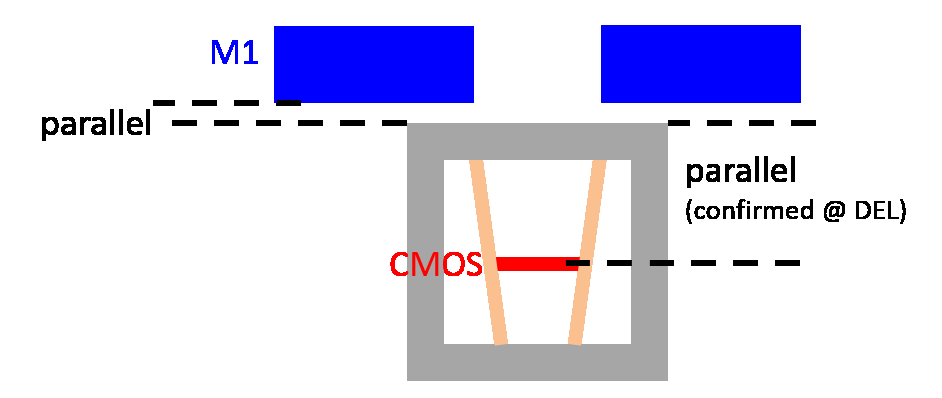
\includegraphics[width=100mm]{MCSinstall.eps}
%\end{center}
%\caption{Sketch of MCS installation}
%\label{fig:MCSinst}
%\end{figure}

% This requirement is not needed any more, because z offset of PFI cannot be measured using MCS image
%\bluetext{
%Additional requirement before shipment:
%The top part of MCS arm and CMOS sensor should be parallel (or angle should be measured).
%}

\begin{itembox}[l]{\suctitle{Success Criteria}}
MCS is mounted to Cassegrain focus with the required accuracy ($\leq$ 45mm offset in x/y direction, and $\leq$ 0.14 degree tilt). 

\bluetext{Required long time to analyze the data?: No.}
\end{itembox}